\chapter{Introduction} \label{chap:introduction}

The aim of this project is to investigate the possibilities of a novel concept of airfoil twist morphing.

%Describe a little bit what is morphing...
The interest in morphing of the aerodynamic surfaces has accompany aerospace history since the beginning. Since the first heavier-than-air flight in 1903, when the Wright Brothers designed and build a powered heavier-than-air aircraft that achieved the  first controlled and sustained flight. Their concept of aircraft did not provide importance to built-in stability but absolute control of the aircraft by the pilot. For this reason, they deliberatively designed their first aircraft with anhedral wing that make it dynamically unstable to perturbations in sideslip but more maneuverable in the lateral direction. In order to achieve roll control, they decided to incorporate a mechanism that would allow the wings to twist by pulling from cables, as it can be seen in Figure \ref{fig:Wright}. This was the first ever use of morphing of an aerodynamic surface for aircraft control. Since them, the necessity of enhanced performance and higher airspeed brought the requirement of stiffer wing structures to avoid aeroelastic instabilities.

\begin{figure}[!htpb]
  \centering
  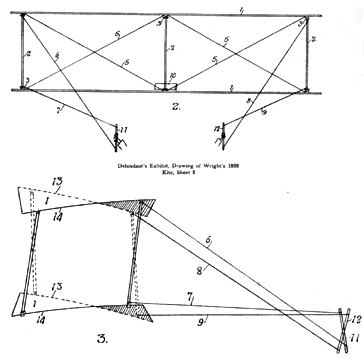
\includegraphics[width=0.6 \textwidth]{state-of-the-art/WrightBrothers1899Kite}
  \caption[Wright Brothers 1899 kite]{Wright 1899 kite: front and side views, with control sticks. Wing-warping is shown in lower view. \cite{Wright}}\label{fig:Wright}
\end{figure}

%Why to used them?
On conventional aircraft, the need to modify the airflow around the airfoil at different flight conditions is achieve through discrete hinged mechanics such as flaps and ailerons. This mechanism performs well in a limited range around the design point while the outside this range, they have a negative influence in the aerodynamics. The necessary discontinuities that these elements produce on the surface, advance the boundary layer transition point from laminar to turbulent regime. Being able to modify the airflow without discontinuities on the surface would come along with notable reductions in parasite drag and therefore in fuel consumption.

%Concept to be test

%Objetives